% Based on docs/ambiguities/template.tex. Build: make questions LECTURE=14
\documentclass[a4paper,12pt]{article}
\usepackage[margin=19mm]{geometry}
\usepackage{amsmath,amssymb,graphicx,xcolor}
\usepackage{fontspec}
\usepackage{xepersian}
\settextfont{XB Roya}
\setlatintextfont{Latin Modern Roman}
\definecolor{ink}{HTML}{173D75}
\graphicspath{{images/}}
\setlength{\parindent}{0pt}
\setlength{\parskip}{5pt}
\linespread{1.12}
\newcommand{\qtitle}[2]{{\Large\bfseries\color{ink} پرسش \lr{#1}: #2}\par}
\newcommand{\answer}{\medskip\textbf{پاسخ یا صورت مورد تأیید و تاریخ:}\par\vspace{18mm}\hrule\medskip}
\begin{document}
{\LARGE\bfseries پرسش‌های ابهام جلسهٔ ۱۴}\par
{\large حلقه‌های ابتدایی؛ جزوهٔ جبر پیشرفتهٔ دکتر خسروی}\par
شمارهٔ صفحه‌ها یک‌مبنا و مربوط به فایل پی‌دی‌اف است. هر سه پرسش برای بازبینی بعدی بازند؛ خوانش‌های کاری موقت و مثالِ موکول‌شده، مانع اتمام دور رونویسی نیستند. پاسخ‌ها در صورت ارائهٔ بعدی ثبت خواهند شد.
\medskip\hrule\medskip

\qtitle{L14-Q01}{شرط اندازه در مثال حلقهٔ ماتریسی}
\textbf{وضعیت:} باز؛ برای بازبینی بعدی؛ ثبت در ۲۰۲۶/۱۰/۲۵.\par
\textbf{نشانی منبع:} نسخهٔ \lr{primary}، صفحهٔ ۲، تذکر دوم؛ مثالِ ساده بودن حلقه و ساده نبودن مدول چپ منظم.
\begin{LTR}\small\texttt{sources/lectures/14 Primitive Rings.pdf}\end{LTR}
\textbf{عبارت منبع:} \(M_n(R)\)، با فرض میدان بودن \(R\)، ایده‌آل دوطرفهٔ غیربدیهی ندارد؛ اما ایده‌آل چپ نابدیهی دارد، مانند ماتریس‌هایی که ستون آخرشان صفر است.
\begin{center}
\includegraphics[width=\linewidth]{L14-Q01-matrix-example.png}\end{center}
\textbf{ابهام و پیامد:} شرطی برای \(n\) در این مثال نوشته نشده است. برای \(n=1\)، خانوادهٔ مذکور فقط ماتریس صفر است و ایده‌آل چپ نابدیهی به دست نمی‌دهد؛ بنابراین ادعای مثال به شرط اندازه نیاز دارد.
\textbf{خوانش کاری در اسلایدها:} شرط \(n\geq2\) صریحاً موقت است؛ پرسش همچنان باز است.

\textbf{پرسش:} آیا شرط \(n\geq2\) را به این مثال اضافه کنم و سپس نابدیهی بودن ایده‌آل چپِ ماتریس‌های با ستون آخر صفر را قطعی بنویسم؟ اگر شرط دیگری مد نظر است، لطفاً مشخص کنید.

\textbf{پاسخ / تصمیم ثبت‌شده:} هنوز دریافت نشده است.
\answer
\newpage

{\large\bfseries پرسش‌های ابهام جلسهٔ ۱۴؛ ادامه}\par
\medskip\hrule\medskip
\qtitle{L14-Q02}{مثال حلقهٔ ساده‌ای که نیمه‌ساده نیست}
\textbf{وضعیت:} باز؛ مثال به بازبینی بعدی موکول است؛ ثبت در ۲۰۲۶/۱۰/۲۵.\par
\textbf{نشانی منبع:} نسخهٔ \lr{primary}، صفحهٔ ۲، تذکر سوم، درست پیش از تعریف حلقهٔ ابتدایی؛ همراه با حاشیهٔ قرمز.
\begin{LTR}\small\texttt{sources/lectures/14 Primitive Rings.pdf}\end{LTR}
\textbf{عبارت منبع:} «ممکن است حلقهٔ سادهٔ \(R\)، نیمه‌ساده هم نباشد»؛ در کروشه آمده است
\[
R=\operatorname{End}_F(V),\qquad \dim_F V=\infty.
\]
مثال در جزوه با یادداشت قرمز «خارج از درس» مشخص شده است.
\begin{center}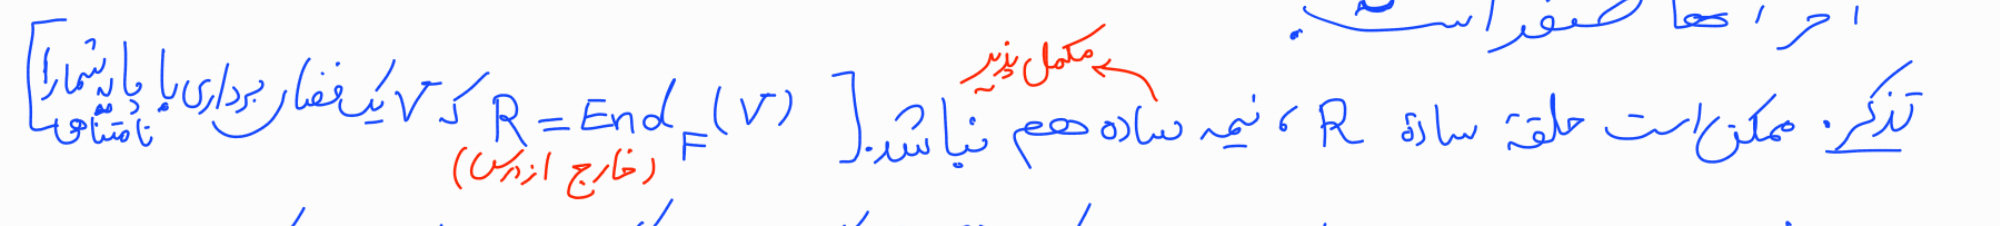
\includegraphics[width=\linewidth]{L14-Q02-endomorphism-example.png}\end{center}
\textbf{دلیل پرسش:} در فضای نامتناهی‌بعد، نگاشت‌های خطی با رتبهٔ متناهی، یک ایده‌آل دوطرفهٔ ناصفر و سره در \(\operatorname{End}_F(V)\) تشکیل می‌دهند؛ پس این حلقه نمی‌تواند نمونهٔ یک حلقهٔ ساده باشد. این توضیح، بررسیِ مثال است و بخشی از متن جزوه نیست.

\textbf{خوانش‌ها / تصمیم‌های ممکن:} ممکن است نام یا وصف حلقه در مثال نیازمند اصلاح باشد؛ یا منظور فقط طرح یک مثالِ نیازمند تکمیل بوده باشد. حذف مثال و حفظ تذکر کلی نیز تصمیمی جداگانه است که نیاز به نظر شما دارد.
\textbf{نحوهٔ پوشش:} تذکر کلی حفظ شده و مثالِ منبع با برچسبِ موکول به بازبینی آمده است؛ مثالِ جایگزین ساخته نشده است.

\textbf{پرسش:} برای این تذکر، چه مثال یا صورت اصلاح‌شده‌ای مد نظر است؟ آیا مثالِ داخل کروشه را حذف کنم و تنها گزارهٔ کلیِ «حلقهٔ ساده لزوماً نیمه‌ساده نیست» را نگه دارم؟

\textbf{پاسخ / تصمیم ثبت‌شده:} هنوز دریافت نشده است.
\answer
\newpage

{\large\bfseries پرسش‌های ابهام جلسهٔ ۱۴؛ ادامه}\par
\medskip\hrule\medskip
\qtitle{L14-Q03}{دو نماد در جهت عکسِ قضیهٔ ایده‌آل ابتدایی}
\textbf{وضعیت:} باز؛ خوانش کاری موقت؛ ثبت در ۲۰۲۶/۱۰/۲۵.\par
\textbf{نشانی منبع:} نسخهٔ \lr{primary}، صفحهٔ ۵؛ فرمول تعریف عمل در بالای صفحه و زیرنویسِ نابودساز در آخرین سطر.
\begin{LTR}\small\texttt{sources/lectures/14 Primitive Rings.pdf}\end{LTR}
\textbf{زمینه:} \(M\) یک \(R\)-مدول ساده است و \(P=\operatorname{Ann}_R(M)\). قرار است \(M\) به یک \(R/P\)-مدول ساده و باوفا تبدیل شود.

\textbf{عبارت نخست:} کنار تعریف عمل، کمیت‌گذار چنین خوانده می‌شود:
\[
(r+P)\cdot m:=r\cdot m,\qquad \forall r\in P.
\]
\begin{center}
\includegraphics[width=.94\linewidth]{L14-Q03-action.png}\end{center}
\textbf{خوانش‌های ممکن و پیامد:} اگر \(r\in P\) باشد، تنها هم‌دستهٔ صفر پوشش داده می‌شود. برای تعریف عملِ تمام عناصر \(R/P\)، انتظار می‌رود \(r\in R\) باشد؛ اما این اصلاح هنوز تأیید نشده است.

\textbf{عبارت دوم:} در پایان، زیرنویس چنین دیده می‌شود:
\(\operatorname{Ann}_{R/I}(M)=0\)، در حالی که در این جهتِ برهان، خارج‌قسمت \(R/P\) است و \(I\) معرفی نشده است.
\begin{center}
\includegraphics[width=.78\linewidth]{L14-Q03-final-subscript.png}\end{center}

\textbf{خوانش کاری در اسلایدها:} هر دو اصلاح زیر و نتیجهٔ برهان، صریحاً موقت‌اند؛ پرسش برای بازبینی بعدی باز می‌ماند.
\textbf{پرسش:} آیا هر دو مورد به صورت زیر مد نظر بوده‌اند؟
\[
\forall r\in R:\quad (r+P)\cdot m:=r\cdot m,
\qquad \operatorname{Ann}_{R/P}(M)=0.
\]
\textbf{پاسخ / تصمیم ثبت‌شده:} هنوز دریافت نشده است.
\answer
\end{document}
